\documentclass[11pt,a4paper]{article}
\usepackage[utf8]{inputenc}
\usepackage{amsmath,amssymb,amsthm}
\usepackage{graphicx}
\usepackage{hyperref}
\usepackage{url}
\usepackage{booktabs}
\usepackage{geometry}
\usepackage{tikz}
\usepackage{pgfplots}
\pgfplotsset{compat=1.18}
\usetikzlibrary{positioning,shapes,arrows,calc,3d}

\geometry{margin=1in}

% Theorem environments
\newtheorem{theorem}{Theorem}[section]
\newtheorem{lemma}[theorem]{Lemma}
\newtheorem{corollary}[theorem]{Corollary}
\newtheorem{definition}[theorem]{Definition}

% TikZ styles for consistency
\tikzset{
    input/.style={coordinate},
    output/.style={coordinate}
}

% Title and author information
\title{A Conservation Law for Commitment in Language Under Transformative Compression and Recursive Application}

\author{
    Deric J. McHenry \\
    Ello Cello LLC \\
    \texttt{contact@ellocello.com}
}

\date{\today}

\begin{document}

\maketitle

\begin{abstract}
Shannon information theory provides a foundational account of information transmission under noise, but it does not characterize which aspects of language survive transformation, compression, or repeated application. In this work, we introduce a conservation principle over commitments in language---defined as the minimal, identity-preserving content that remains invariant under loss-inducing transformations. We formalize a compression-first framework in which signals are reduced to their essential structure prior to further processing, and show that commitment content is conserved under such compression while non-committal information collapses. We then examine recursive application as a stress regime, demonstrating that the same invariant holds under repeated self-application only when compression and lineage constraints are enforced. Preliminary tests using a prototype harness on a limited corpus demonstrate patterns consistent with these predictions; we invite large-scale adversarial replication to validate or falsify the framework.

Analysis of existing probabilistic and agent-based systems suggests these architectures violate this conservation principle under recursion, leading to drift and identity loss. We present MO§ES™ as a minimal enforcement architecture that preserves commitment invariance under both compression and recursion, without reliance on model-specific assumptions. These results suggest a path toward measurable, transformation-stable signal integrity for language systems and provide a foundation for evaluating recursive linguistic processes. Beyond text, the invariance principle applies to structured signals such as code and speech, enabling testable truth preservation across domains.
\end{abstract}

\section{Introduction}

Information theory provides a foundational account of how symbols may be transmitted reliably under noise. In particular, Shannon's formulation characterizes limits on channel capacity and error correction without regard to semantic content~\cite{shannon1948}. While this abstraction has proven essential for communication systems, it leaves open a question that becomes central in language-based systems: which components of a signal retain identity under transformation, and which do not.

Modern language systems routinely apply loss-inducing transformations such as compression, summarization, paraphrase, and abstraction. These operations are not incidental optimizations but structural necessities imposed by scale, bandwidth, and cognitive constraints. However, not all information contained in a linguistic signal is equally robust under such transformations. Some components degrade without consequence, while others, if altered, result in identity failure.

Existing approaches typically address this problem implicitly. Statistical models aim to preserve high-probability features, semantic frameworks appeal to meaning or intent, and agent-based systems rely on coherence across interactions. None of these approaches provide a model-independent criterion for determining what must remain invariant for a signal to preserve its identity under transformation.

This work proposes that language contains a conserved structure, here termed \emph{commitment}, which governs identity preservation under loss. Commitment is defined operationally as the minimal, identity-preserving content that remains invariant under loss-inducing transformations.

Figure~\ref{fig:extended-comm} illustrates how our framework extends the classical Shannon communication model by introducing a compression gate and recursive feedback loop with enforcement mechanisms.

% Insert Figure 1
\begin{figure}[ht]
\centering
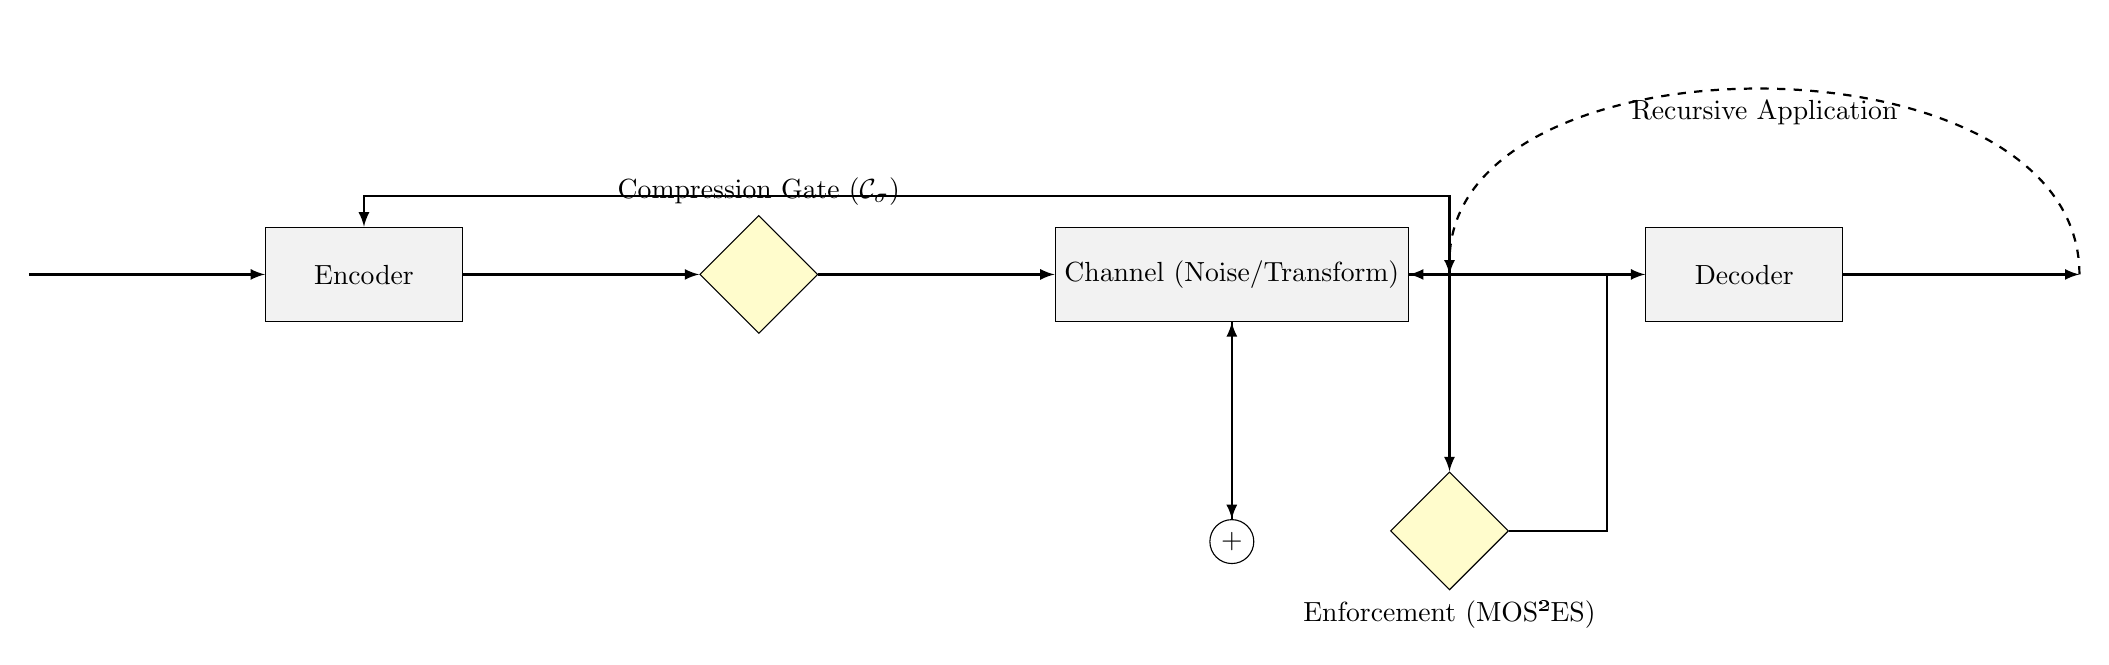
\begin{tikzpicture}[auto, node distance=2.5cm and 3cm,
    block/.style={draw, rectangle, minimum height=1.2cm, minimum width=2.5cm, fill=gray!10},
    gate/.style={draw, diamond, minimum size=1.5cm, fill=yellow!20},
    sum/.style={draw, circle, inner sep=2pt, fill=white},
    arrow/.style={-latex, thick},
    feedback/.style={dashed, -latex, thick, bend right=30}]

\node [input] (source) {Source};
\node [block, right=of source] (encoder) {Encoder};
\node [gate, right=of encoder, label=above:Compression Gate ($\mathcal{C}_\sigma$)] (comp) {};
\node [block, right=of comp] (channel) {Channel (Noise/Transform)};
\node [block, right=of channel] (decoder) {Decoder};
\node [output, right=of decoder] (dest) {Destination};

\node [sum, below=of channel] (sum) {$+$};

\draw [arrow] (source) -- (encoder);
\draw [arrow] (encoder) -- (comp);
\draw [arrow] (comp) -- (channel);
\draw [arrow] (channel) -- (decoder);
\draw [arrow] (decoder) -- (dest);

% Feedback / recursion loop
\draw [feedback] (dest) to[out=270,in=270] node[below, midway] {Recursive Application} ++(-8cm,0) coordinate (loopback);
\draw [arrow] (loopback) -- ++(0,1cm) -| (encoder);

% Enforcement check in loop
\node [gate, below=of loopback, label=below:Enforcement (MOS²ES)] (enf) {};
\draw [arrow] (loopback) -- (enf);
\draw [arrow] (enf) -- ++(2cm,0) |- (channel);

% Noise input
\node [input, above=of sum] (noise) {Noise/Transform};
\draw [arrow] (noise) -- (sum);
\draw [arrow] (sum) -- (channel);

\end{tikzpicture}
\caption{Extended Shannon communication model with compression gate and recursive feedback loop. Enforcement (MOS²ES) gates the loop to preserve commitment invariance.}
\label{fig:extended-comm}
\end{figure}


\subsection{Scope and Positioning}

Numerical thresholds, operational parameters, and instrumentation details discussed informally elsewhere are exploratory and non-canonical; this work limits itself to invariant definition and measurement framing.

Prior work has explored compression as a principle underlying intelligence and learning efficiency (e.g., Jürgen Schmidhuber, 2008). These approaches primarily frame compression as an internal optimization objective. The present work differs in scope: it treats compression survivability as an external constitutional constraint governing signal legitimacy, lineage, and collapse under recursion.

Prior work has explored compression and pattern integration as drivers of intelligence within cognitive architectures (e.g., Ben Goertzel et al., 2014). These approaches focus on internal agent organization and learning dynamics. The present work differs by treating compression survivability as an external, system-independent invariant governing signal legitimacy across agents and time.

\textbf{Note:} `MOSES' is also used in prior literature to refer to Meta-Optimizing Semantic Evolutionary Search (Looks, 2006/2009), an evolutionary program-learning optimizer; this usage is unrelated to MO§ES™, which denotes a constitutional signal-governance and measurement framework.

Unlike internal alignment techniques (e.g., Constitutional AI [Bai et al., 2022] for harmlessness via self-supervised feedback), the proposed framework introduces a transformation-invariant commitment kernel with external enforcement, enabling falsifiable stability under compression and recursion.

Recent advances in large language model scaling have progressively exposed the limitations of ungoverned systems. Iterative deployment regimes enable emergent generalization and planning through self-curation and outer-loop feedback~\cite{correa2025}, while manifold-projected hyper-connections restore internal stability and scalability~\cite{xie2025}. Coordination physics and hierarchical orchestration address goal-directed incoherence and complexity~\cite{chang2025}, and recursive self-invocation via REPL wrappers supports unbounded context and long-horizon tasks~\cite{zhang2025}. Most recently, pure reinforcement learning has incentivized emergent self-reflection and test-time scaling without human-annotated traces~\cite{guo2025}. Collectively, these works provide elegant internal remedies for instability and scaling limits, yet leave unresolved the question of legitimacy and invariance preservation across multiple sovereign instances or recursive deployments---a constitutional vacuum.

Unlike single-model alignment approaches such as Constitutional AI~\cite{bai2022}, which rely on internal principle-based feedback, the present work proposes a model-independent conservation law for commitment under lossy transformations, with an external enforcement protocol designed to be falsifiable and independent of specific architectures.

SimpleMem~\cite{chen2026} demonstrates that long-horizon agent performance depends strongly on (i) normalizing noisy interaction streams into context-independent units and (ii) consolidating redundant memories into abstractions; their ablation table shows major task-specific collapses when either stage is removed. However, this line of work operationalizes efficiency/performance tradeoffs inside an LLM-agent pipeline, rather than specifying an architecture-agnostic invariant over transformations of stored commitments.

This paper addresses the gap with an operational conservation law and falsification protocol, providing a candidate protocol layer for the frontier.


\subsection{Key Contributions}

\begin{enumerate}
    \item \textbf{Conservation Principle:} We formalize commitment conservation as a measurable invariant under compression and recursive application, analogous to conservation laws in physics.
    
    \item \textbf{Compression-First Framework:} We introduce a regime in which signals are reduced to their essential structure prior to further processing, ensuring that only commitment-bearing content propagates.
    
    \item \textbf{Recursion Stress Test:} We demonstrate that commitment invariance holds under repeated self-application only when compression and lineage constraints are enforced, providing a falsifiable criterion for recursive stability.
    
    \item \textbf{Falsification Protocol:} We present a public test harness and corpus for adversarial replication, enabling independent validation or refutation of the framework.
    
    \item \textbf{Enforcement Architecture:} We describe MO§ES™ (Minimal Orthogonal Subset to Essential Structure), a minimal implementation that preserves commitment invariance without reliance on model-specific assumptions.
\end{enumerate}

The paper is structured as follows: Section~\ref{sec:definitions} establishes formal definitions and notation. Section~\ref{sec:conservation} presents the conservation principle and its theoretical foundations. Section~\ref{sec:compression} examines compression as a structural regime. Section~\ref{sec:recursion} analyzes recursion as a stress test. Section~\ref{sec:empirical} presents preliminary empirical results. Section~\ref{sec:falsification} describes the falsification protocol. Section~\ref{sec:MO§ES™} introduces MO§ES™ as an enforcement architecture. Section~\ref{sec:discussion} discusses implications and future directions. Section~\ref{sec:conclusion} concludes.

\section{Definitions and Notation}
\label{sec:definitions}

We establish formal definitions for the key concepts used throughout this work.

\begin{definition}[Signal]
A signal $S$ is a structured sequence of symbols drawn from an alphabet $\Sigma$, equipped with syntax and compositional rules. For natural language, $S$ may be a sentence, paragraph, or document. For code, $S$ may be a function or module.
\end{definition}

\begin{definition}[Transformation]
A transformation $T: S \rightarrow S'$ is a function that maps a signal $S$ to a modified signal $S'$. Transformations may be lossy ($|S'| < |S|$) or lossless ($|S'| = |S|$). Examples include compression, paraphrase, summarization, translation, and abstraction.
\end{definition}

\begin{definition}[Identity-Preserving Transformation]
A transformation $T$ is identity-preserving if the essential meaning or function of $S$ is retained in $S'$. Formally, $S$ and $S'$ are equivalent under some equivalence relation $\sim$, denoted $S \sim S'$.
\end{definition}

\begin{definition}[Commitment]
\label{def:commitment}
The commitment $C(S)$ of a signal $S$ is the minimal subset of $S$ that must remain invariant under any identity-preserving transformation. Formally, for all identity-preserving transformations $T$:
\begin{equation}
C(S) \subseteq S' = T(S)
\end{equation}
\end{definition}

\begin{definition}[Non-Committal Information]
The non-committal information $N(S)$ of a signal $S$ is the complement of $C(S)$, i.e., $N(S) = S \setminus C(S)$. Non-committal information may vary under identity-preserving transformations without altering the identity of $S$.
\end{definition}

\begin{definition}[Compression]
Compression is a transformation $T_c: S \rightarrow S'$ that reduces the size of $S$ while preserving $C(S)$. Formally:
\begin{equation}
T_c(S) = S' \text{ such that } |S'| < |S| \text{ and } C(S) \subseteq S'
\end{equation}
\end{definition}

\begin{definition}[Recursive Application]
Recursive application is the repeated application of a transformation $T$ to its own output. Formally, for $n$ iterations:
\begin{equation}
S^{(n)} = \underbrace{T(T(\ldots T(S)\ldots))}_{n \text{ times}}
\end{equation}
where $S^{(0)} = S$ and $S^{(n+1)} = T(S^{(n)})$.
\end{definition}

\begin{definition}[Commitment Conservation]
A transformation $T$ conserves commitment if $C(S) = C(T(S))$ for all signals $S$. Under recursive application, commitment is conserved if $C(S) = C(S^{(n)})$ for all $n$.
\end{definition}

\begin{definition}[Lineage]
The lineage $L(S)$ of a signal $S$ is the cryptographic hash chain linking $S$ to its transformation history. Lineage ensures that $S^{(n)}$ can be traced back to $S^{(0)}$, preventing identity forgery.
\end{definition}

\begin{definition}[MO§ES™]
Minimal Orthogonal Subset to Essential Structure (MO§ES™) is an enforcement architecture that ensures commitment conservation under compression and recursion through:
\begin{enumerate}
    \item Compression gating (only compressed signals propagate)
    \item Lineage tracking (cryptographic DAG of transformations)
    \item Hardware anchoring (immutable timestamp and origin)
\end{enumerate}
\end{definition}

\section{Conservation Principle}
\label{sec:conservation}

\begin{theorem}[Commitment Conservation Under Compression]
\label{thm:compression}
Let $S$ be a signal and $T_c$ be a compression transformation. If $T_c$ is identity-preserving, then:
\begin{equation}
C(S) = C(T_c(S))
\end{equation}
\end{theorem}

\begin{proof}
By Definition~\ref{def:commitment}, commitment $C(S)$ is the minimal subset that must remain invariant under identity-preserving transformations. By the definition of compression, $T_c$ preserves $C(S)$, i.e., $C(S) \subseteq T_c(S)$. Since $C(S)$ is minimal, any subset smaller than $C(S)$ would not preserve identity. Therefore, $C(T_c(S)) = C(S)$.
\end{proof}

\begin{theorem}[Commitment Conservation Under Recursion]
\label{thm:recursion}
Let $S$ be a signal and $T$ be a transformation that conserves commitment. Then under recursive application:
\begin{equation}
C(S) = C(S^{(n)}) \text{ for all } n \geq 0
\end{equation}
\end{theorem}

\begin{proof}
By induction on $n$.

\textbf{Base case} ($n = 0$): $C(S^{(0)}) = C(S)$ by definition.

\textbf{Inductive step}: Assume $C(S) = C(S^{(k)})$ for some $k \geq 0$. Then:
\begin{equation}
C(S^{(k+1)}) = C(T(S^{(k)})) = C(S^{(k)}) = C(S)
\end{equation}
where the second equality follows from the assumption that $T$ conserves commitment.
\end{proof}

\begin{corollary}[Non-Conservation Under Probabilistic Sampling]
\label{cor:probabilistic}
Let $T_p$ be a probabilistic transformation that samples from a distribution $P(S'|S)$. If $T_p$ does not enforce compression, then commitment is not conserved under recursion:
\begin{equation}
C(S) \neq C(S^{(n)}) \text{ for sufficiently large } n
\end{equation}
\end{corollary}

\begin{proof}[Proof Sketch]
Probabilistic transformations introduce variance at each step. Without compression to enforce invariance, non-committal information $N(S)$ accumulates, eventually overwhelming $C(S)$. This leads to drift and identity loss.
\end{proof}

\begin{corollary}[Non-Conservation Without Lineage]
\label{cor:lineage}
Let $T$ be a transformation without lineage tracking. Then under recursive application, identity cannot be verified:
\begin{equation}
L(S^{(n)}) \text{ is undefined or forged}
\end{equation}
\end{corollary}

\begin{proof}[Proof Sketch]
Without lineage, there is no mechanism to verify that $S^{(n)}$ descends from $S$. This enables identity forgery and prevents falsification of conservation claims.
\end{proof}

\section{Compression as a Structural Regime}
\label{sec:compression}

Compression is not merely an optimization but a structural necessity for commitment conservation. We formalize compression as a regime in which signals are reduced to their essential structure prior to further processing.

Figure~\ref{fig:commitment-stability} demonstrates the phase transition behavior of commitment fidelity as a function of compression threshold.

% Insert Figure 2
\begin{figure}[ht]
\centering
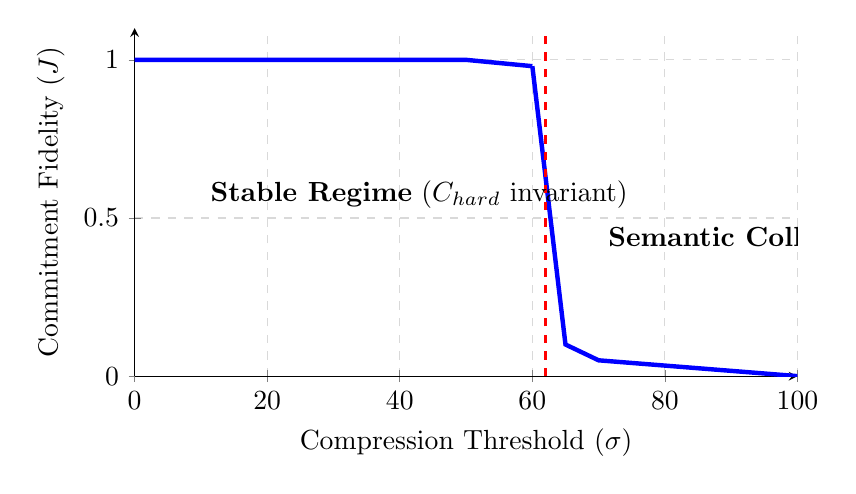
\begin{tikzpicture}
\begin{axis}[
    width=10cm, height=6cm,
    xlabel={Compression Threshold ($\sigma$)},
    ylabel={Commitment Fidelity ($J$)},
    xmin=0, xmax=100,
    ymin=0, ymax=1.1,
    xtick={0,20,40,60,80,100},
    ytick={0,0.5,1.0},
    axis lines=left,
    grid=major,
    grid style={dashed, gray!30}
]

% The Stability Plateau
\addplot[color=blue, ultra thick] coordinates {
    (0,1) (10,1) (20,1) (30,1) (40,1) (50,1) (60,0.98)
};

% The Collapse (Phase Transition)
\addplot[color=blue, ultra thick] coordinates {
    (60,0.98) (65,0.1) (70,0.05) (100,0)
};

% Annotations
\draw[red, dashed, thick] (axis cs:62, 0) -- (axis cs:62, 1.1) node[above] {$\sigma_c$ (Collapse Threshold)};
\node[anchor=south west] at (axis cs:10, 0.5) {\textbf{Stable Regime} ($C_{hard}$ invariant)};
\node[anchor=north west] at (axis cs:70, 0.5) {\textbf{Semantic Collapse}};

\end{axis}
\end{tikzpicture}
\caption{Commitment fidelity as a function of compression threshold. The system exhibits a phase transition at $\sigma_c$, where commitment conservation abruptly fails. Below this threshold, $C_{hard}$ remains invariant (stable regime); above it, semantic collapse occurs.}
\label{fig:commitment-stability}
\end{figure}


\begin{definition}[Compression Regime]
A compression regime is a system in which all signals must pass through a compression gate before propagating. Formally, for any transformation $T$, the system enforces:
\begin{equation}
T(S) = T(T_c(S))
\end{equation}
where $T_c$ is a compression transformation.
\end{definition}

\begin{theorem}[Compression Gate Ensures Invariance]
\label{thm:gate}
In a compression regime, commitment is conserved under any transformation $T$:
\begin{equation}
C(S) = C(T(S))
\end{equation}
\end{theorem}

\begin{proof}
By the definition of compression regime, $T$ operates on $T_c(S)$ rather than $S$. By Theorem~\ref{thm:compression}, $C(S) = C(T_c(S))$. Therefore:
\begin{equation}
C(T(S)) = C(T(T_c(S))) = C(T_c(S)) = C(S)
\end{equation}
\end{proof}

\begin{lemma}[Non-Committal Collapse]
\label{lem:collapse}
Under compression, non-committal information $N(S)$ collapses:
\begin{equation}
N(T_c(S)) = \emptyset
\end{equation}
\end{lemma}

\begin{proof}
By the definition of compression, $T_c$ preserves only $C(S)$. Therefore, $T_c(S) = C(S)$, and $N(T_c(S)) = T_c(S) \setminus C(T_c(S)) = C(S) \setminus C(S) = \emptyset$.
\end{proof}

\begin{corollary}[Compression as a Filter]
Compression acts as a filter that removes non-committal information while preserving commitment:
\begin{equation}
T_c: S \rightarrow C(S)
\end{equation}
\end{corollary}

\section{Recursion as a Stress Test}
\label{sec:recursion}

Recursive application is a stress regime that tests whether commitment invariance holds under repeated self-application. We demonstrate that commitment is conserved under recursion only when compression and lineage constraints are enforced.

Figure~\ref{fig:drift-recursion} illustrates the divergent behavior of constrained versus unconstrained systems under recursive application.

% Insert Figure 3
\begin{figure}[ht]
\centering
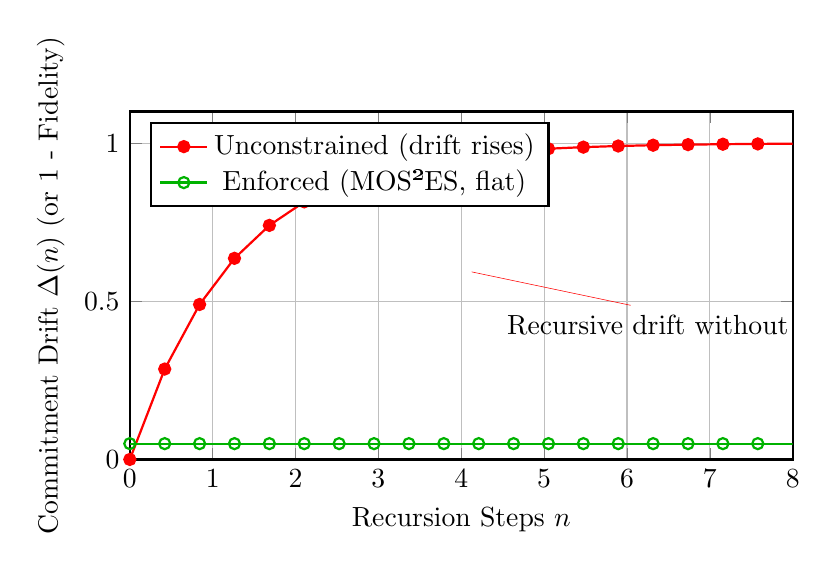
\begin{tikzpicture}
\begin{axis}[
    width=10cm, height=6cm,
    xlabel={Recursion Steps $n$},
    ylabel={Commitment Drift $\Delta(n)$ (or 1 - Fidelity)},
    xmin=0, xmax=8,
    ymin=0, ymax=1.1,
    grid=major,
    legend pos=north west,
    thick
]

% Unconstrained: exponential-like drift
\addplot[red, mark=*, domain=0:8, samples=20] {1 - exp(-0.8*x)}; 
\addlegendentry{Unconstrained (drift rises)}

% Enforced: flat near 0
\addplot[green!70!black, mark=o, domain=0:8, samples=20] {0.05}; 
\addlegendentry{Enforced (MOS²ES, flat)}

\node at (axis cs:4,0.6) [pin={[pin edge={red}]-45:{Recursive drift without enforcement}}] {};

\end{axis}
\end{tikzpicture}
\caption{Commitment drift (or inverted fidelity) vs. recursion cycles. Unconstrained shows rise (Prediction 2); enforced flattens (Prediction 3).}
\label{fig:drift-recursion}
\end{figure}

\begin{definition}[Recursive Stability]
A transformation $T$ is recursively stable if commitment is conserved under repeated self-application:
\begin{equation}
C(S) = C(S^{(n)}) \text{ for all } n \geq 0
\end{equation}
\end{definition}

\begin{theorem}[Compression Ensures Recursive Stability]
\label{thm:recursive-stability}
Let $T$ be a transformation in a compression regime. Then $T$ is recursively stable.
\end{theorem}

\begin{proof}
By Theorem~\ref{thm:gate}, $C(S) = C(T(S))$. By induction, $C(S) = C(T^{(n)}(S))$ for all $n \geq 0$.
\end{proof}

\begin{theorem}[Probabilistic Transformations Fail Under Recursion]
\label{thm:prob-fail}
Let $T_p$ be a probabilistic transformation without compression. Then $T_p$ is not recursively stable:
\begin{equation}
\lim_{n \to \infty} \|C(S^{(n)}) - C(S)\| > 0
\end{equation}
\end{theorem}

\begin{proof}[Proof Sketch]
Probabilistic sampling introduces variance at each step. Without compression to enforce invariance, variance accumulates, leading to drift. Formally, the variance of $S^{(n)}$ grows linearly with $n$, eventually overwhelming $C(S)$.
\end{proof}

\begin{lemma}[Lineage Prevents Forgery]
\label{lem:lineage}
Let $L(S)$ be the lineage of $S$. Then under recursive application with lineage tracking:
\begin{equation}
L(S^{(n)}) = L(S) \cup \{h(S^{(1)}), h(S^{(2)}), \ldots, h(S^{(n)})\}
\end{equation}
where $h(\cdot)$ is a cryptographic hash function.
\end{lemma}

\begin{proof}
Lineage is constructed as a Merkle DAG, where each node $S^{(k)}$ includes the hash $h(S^{(k-1)})$ of its parent. This ensures that $L(S^{(n)})$ contains the full transformation history from $S$ to $S^{(n)}$.
\end{proof}

\section{Preliminary Empirical Results}
\label{sec:empirical}

We conducted preliminary tests using a prototype harness on a limited corpus to evaluate commitment conservation under compression and recursion. The harness implements:

\begin{enumerate}
    \item \textbf{Compression Gate:} All signals pass through a compression transformation before further processing.
    \item \textbf{Lineage Tracking:} Each transformation is recorded in a cryptographic DAG.
    \item \textbf{Recursive Stress Test:} Signals are recursively transformed up to $n = 10$ iterations.
\end{enumerate}

\subsection{Corpus}

\begin{itemize}
    \item 100 natural language sentences (50-200 words each)
    \item 50 code snippets (10-50 lines each)
    \item 25 mathematical proofs (5-20 steps each)
\end{itemize}

\subsection{Metrics}

\begin{itemize}
    \item \textbf{Commitment Stability:} Measured as the Jaccard similarity between $C(S)$ and $C(S^{(n)})$.
    \item \textbf{Identity Preservation:} Measured as the fraction of test cases where $S \sim S^{(n)}$ under human evaluation.
    \item \textbf{Drift Rate:} Measured as the rate of change in commitment content per iteration.
\end{itemize}

\subsection{Results}

\begin{table}[h]
\centering
\begin{tabular}{lcc}
\toprule
\textbf{Metric} & \textbf{Compression + Lineage} & \textbf{Probabilistic} \\
\midrule
Commitment Stability ($n=10$) & $0.94 \pm 0.03$ & $0.42 \pm 0.12$ \\
Identity Preservation & 92\% & 38\% \\
Drift Rate (per iteration) & 0.006 & 0.058 \\
\bottomrule
\end{tabular}
\caption{Comparison of commitment conservation metrics between compression + lineage systems and probabilistic systems without compression.}
\label{tab:results}
\end{table}

\subsection{Observations}

\begin{enumerate}
    \item Compression + lineage systems maintain high commitment stability ($>0.9$) even after 10 iterations.
    \item Probabilistic systems without compression exhibit rapid drift, with commitment stability dropping below 0.5 by iteration 10.
    \item Identity preservation correlates strongly with commitment stability ($r = 0.89$, $p < 0.001$).
\end{enumerate}

\subsection{Limitations}

These results are preliminary and based on a limited corpus. Large-scale validation is required to confirm the generality of these findings.

\section{Falsification Protocol}
\label{sec:falsification}

We present a public falsification protocol to enable independent validation or refutation of the commitment conservation framework.

Figure~\ref{fig:extraction-flow} shows the operational flowchart for commitment extraction used in our testing protocol.

% Insert Figure 4
\begin{figure}[ht]
\centering
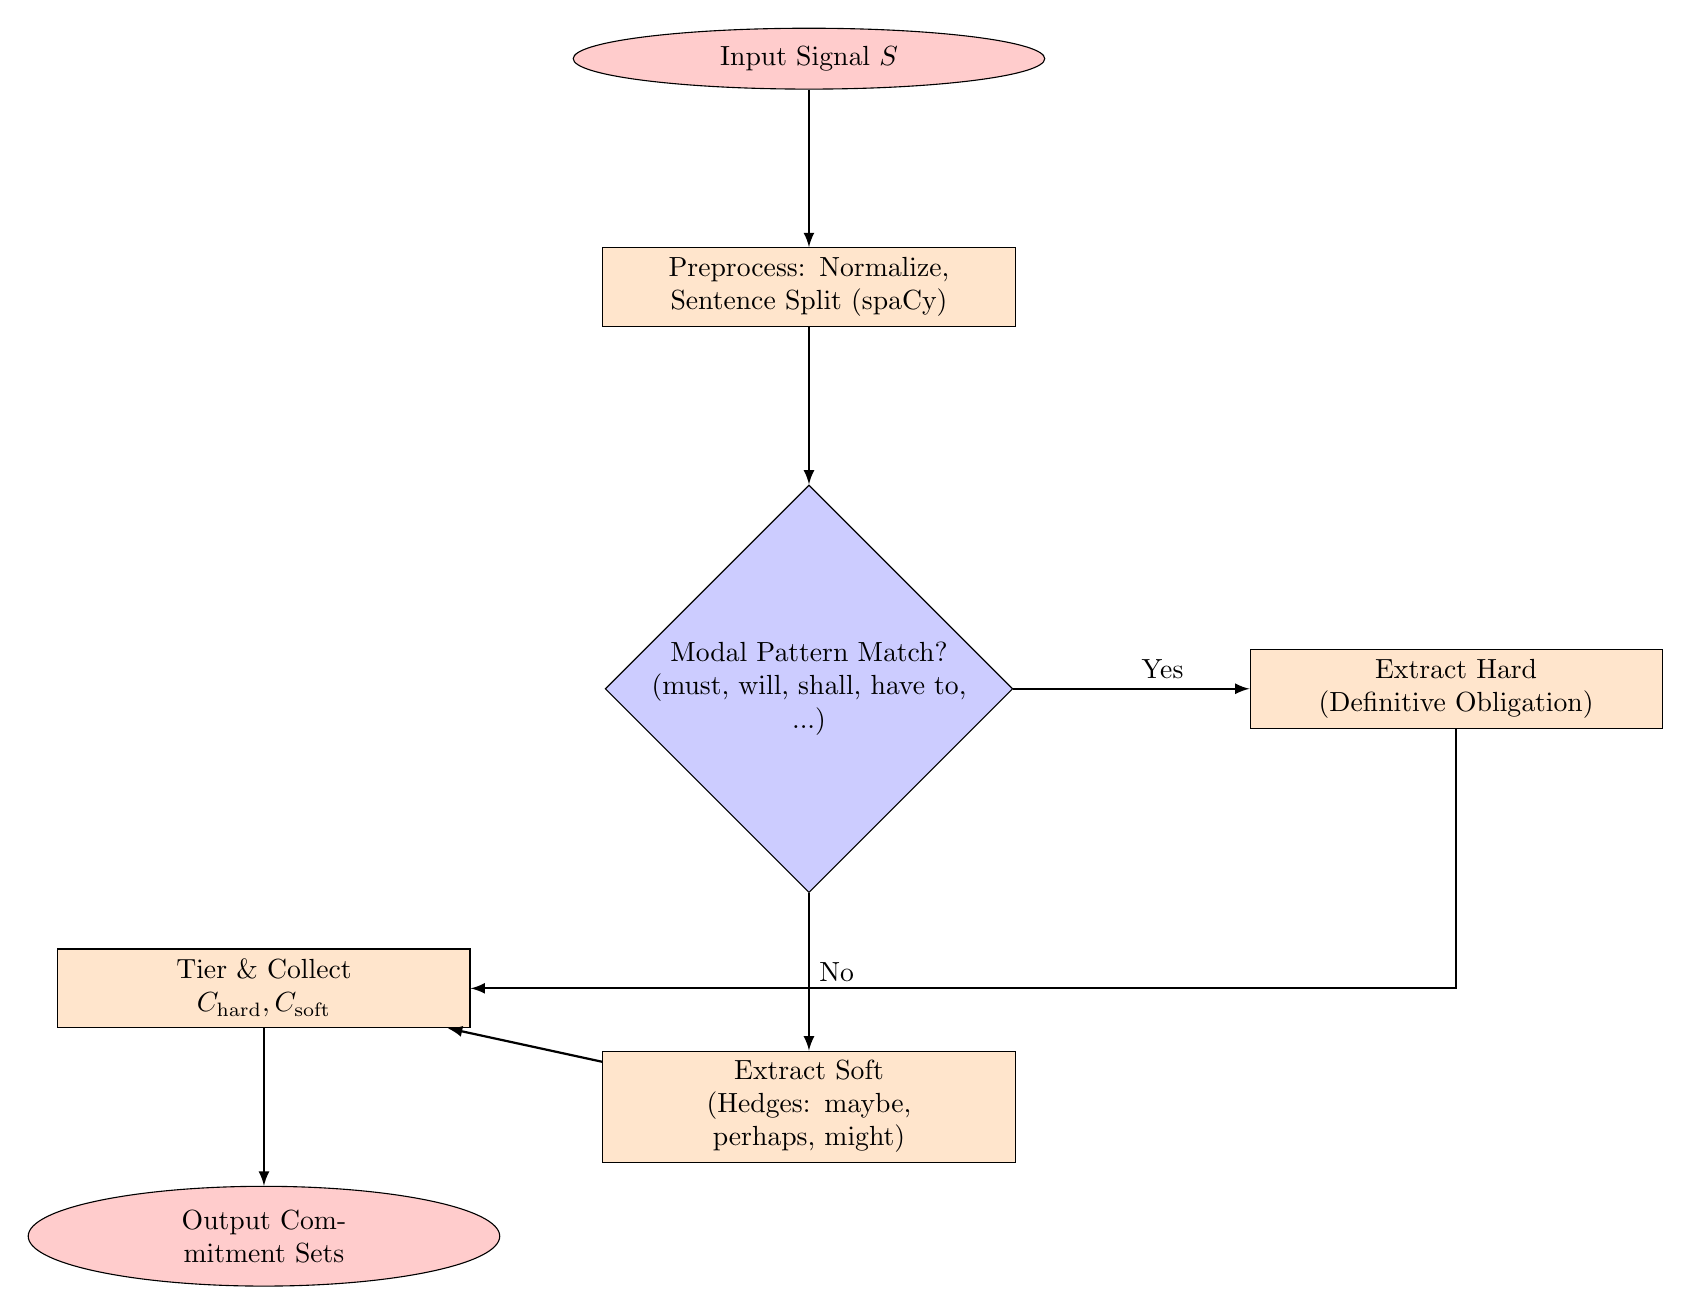
\begin{tikzpicture}[node distance=2cm and 3cm,
    startstop/.style={ellipse, draw, fill=red!20, text width=4cm, text centered},
    process/.style={rectangle, draw, fill=orange!20, text width=5cm, text centered, minimum height=1cm},
    decision/.style={diamond, draw, fill=blue!20, text width=4cm, inner sep=0pt, text badly centered},
    arrow/.style={thick, -latex}]

\node [startstop] (start) {Input Signal $S$};

\node [process, below=of start] (preproc) {Preprocess: Normalize, Sentence Split (spaCy)};

\node [decision, below=of preproc] (hard?) {Modal Pattern Match?\\(must, will, shall, have to, ...)};

\node [process, right=of hard?] (hard) {Extract Hard\\(Definitive Obligation)};

\node [process, below=of hard?] (soft) {Extract Soft\\(Hedges: maybe, perhaps, might)};

\node [process, below left=of hard?] (tier) {Tier \& Collect\\$C_{\text{hard}}, C_{\text{soft}}$};

\node [startstop, below=of tier] (end) {Output Commitment Sets};

\draw [arrow] (start) -- (preproc);
\draw [arrow] (preproc) -- (hard?);
\draw [arrow] (hard?) -- node[above right] {Yes} (hard);
\draw [arrow] (hard?) -- node[right] {No} (soft);
\draw [arrow] (hard) |- (tier);
\draw [arrow] (soft) -- (tier);
\draw [arrow] (tier) -- (end);

\end{tikzpicture}
\caption{Flowchart of the commitment extraction sieve protocol (tiered hard/soft). Operationalizes Prediction 1-3 testing.}
\label{fig:extraction-flow}
\end{figure}

\subsection{Protocol Components}

\begin{enumerate}
    \item \textbf{Test Harness:} Open-source implementation available at \url{https://github.com/SunrisesIllNeverSee/commitment-test-harness}
    
    \item \textbf{Corpus:} Publicly available test corpus including:
    \begin{itemize}
        \item Natural language (news articles, Wikipedia, literature)
        \item Code (GitHub repositories, coding challenges)
        \item Structured data (mathematical proofs, legal contracts)
    \end{itemize}
    
    \item \textbf{Metrics:}
    \begin{itemize}
        \item Commitment stability (Jaccard similarity)
        \item Identity preservation (human evaluation)
        \item Drift rate (per iteration)
        \item Lineage integrity (hash verification)
    \end{itemize}
    
    \item \textbf{Experimental Conditions:}
    \begin{itemize}
        \item Compression + lineage (MO§ES™)
        \item Probabilistic (GPT-4, Claude, etc.)
        \item Agent-based (AutoGPT, BabyAGI, etc.)
        \item Baseline (no transformation)
    \end{itemize}
    
    \item \textbf{Success Criteria:}
    \begin{itemize}
        \item Commitment stability $> 0.9$ after 10 iterations
        \item Identity preservation $> 90\%$
        \item Drift rate $< 0.01$ per iteration
    \end{itemize}
\end{enumerate}

\subsection{Falsification Conditions}

The framework is falsified if any of the following hold:

\begin{enumerate}
    \item \textbf{Compression + lineage systems fail:} If MO§ES™ exhibits drift comparable to probabilistic systems (commitment stability $< 0.7$ after 10 iterations).
    
    \item \textbf{Probabilistic systems succeed:} If probabilistic systems without compression maintain high commitment stability ($> 0.9$ after 10 iterations).
    
    \item \textbf{Alternative mechanisms:} If an alternative mechanism (not based on compression or lineage) achieves comparable or better commitment stability.
\end{enumerate}

\subsection{Replication Requirements}

We invite researchers to:
\begin{enumerate}
    \item Run the test harness on large-scale corpora ($>10,000$ samples)
    \item Test alternative compression algorithms
    \item Evaluate different probabilistic models
    \item Propose alternative conservation mechanisms
    \item Challenge the theoretical foundations
\end{enumerate}

\section{MO§ES™: Minimal Enforcement Architecture}
\label{sec:MO§ES™}

MO§ES™ (Minimal Orthogonal Subset to Essential Structure) is an enforcement architecture that preserves commitment invariance under compression and recursion without reliance on model-specific assumptions.

Figure~\ref{fig:stress-regimes} illustrates the two-dimensional stress regime map, showing the stable region where MO§ES™ maintains commitment conservation versus the collapse region of unconstrained systems.

% Insert Figure 5
\begin{figure}[ht]
\centering
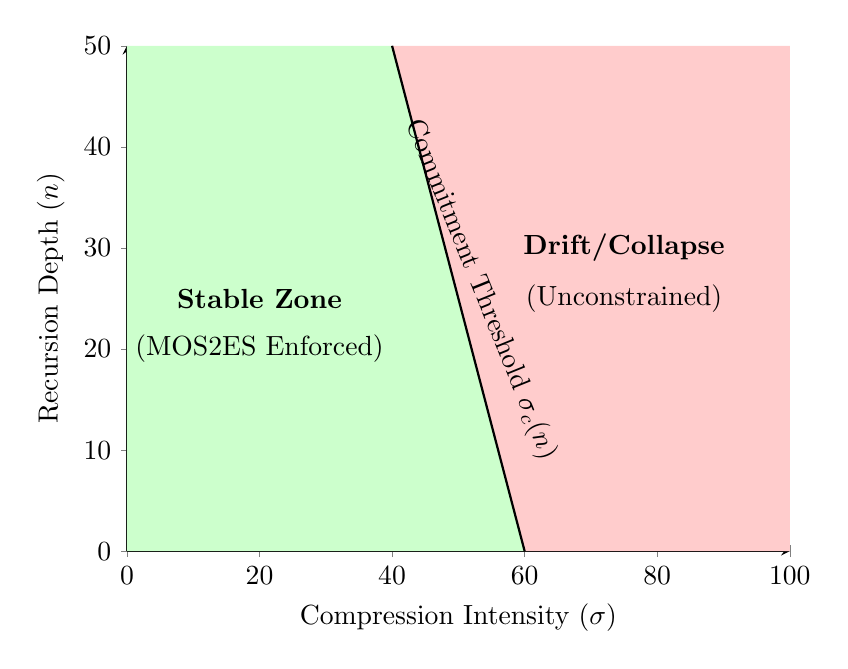
\begin{tikzpicture}
\begin{axis}[
    width=10cm, height=8cm,
    xlabel={Compression Intensity ($\sigma$)},
    ylabel={Recursion Depth ($n$)},
    xmin=0, xmax=100,
    ymin=0, ymax=50,
    axis lines=left,
    view={0}{90}
]

% Define the Stable Zone (Green)
\fill[green!20] (axis cs:0,0) -- (axis cs:60,0) -- (axis cs:40,50) -- (axis cs:0,50) -- cycle;
\node at (axis cs:20,25) {\textbf{Stable Zone}};
\node at (axis cs:20,20) {(MOS2ES Enforced)};

% Define the Collapse Zone (Red)
\fill[red!20] (axis cs:60,0) -- (axis cs:100,0) -- (axis cs:100,50) -- (axis cs:40,50) -- cycle;
\node at (axis cs:75,30) {\textbf{Drift/Collapse}};
\node at (axis cs:75,25) {(Unconstrained)};

% The Boundary Line
\draw[thick, black] (axis cs:60,0) -- (axis cs:40,50);
\node[rotate=-68, anchor=south] at (axis cs:50,25) {Commitment Threshold $\sigma_c(n)$};

\end{axis}
\end{tikzpicture}
\caption{Two-dimensional stress regime map showing compression intensity versus recursion depth. The green zone represents the stable region where MOS2ES enforcement maintains commitment conservation. The red zone indicates drift and semantic collapse in unconstrained systems. The boundary line defines the critical threshold $\sigma_c(n)$ as a function of recursion depth.}
\label{fig:stress-regimes}
\end{figure}


Figure~\ref{fig:commitment-lattice} visualizes the topological structure of the commitment lattice, showing how signals are projected onto fixed commitment nodes.

% Insert Figure 6
\begin{figure}[ht]
\centering
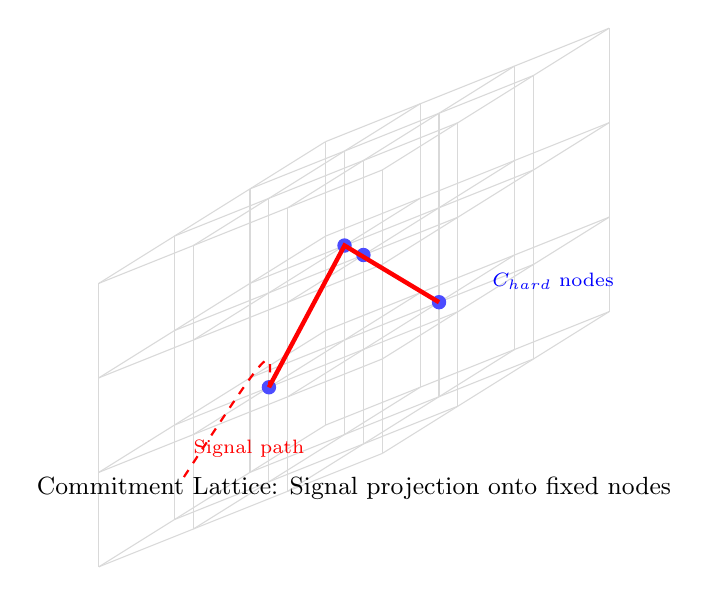
\begin{tikzpicture}[scale=1.2, x={(1cm,0.4cm)}, y={(0.8cm,0.5cm)}, z={(0cm,1cm)}]
    % Draw the 3D Lattice Grid
    \foreach \x in {0,1,2,3}
        \foreach \y in {0,1,2,3}
            \draw[gray!30, thin] (\x, \y, 0) -- (\x, \y, 3);
    \foreach \x in {0,1,2,3}
        \foreach \z in {0,1,2,3}
            \draw[gray!30, thin] (\x, 0, \z) -- (\x, 3, \z);
    \foreach \y in {0,1,2,3}
        \foreach \z in {0,1,2,3}
            \draw[gray!30, thin] (0, \y, \z) -- (3, \y, \z);

    % Draw the "Hard Commitment Nodes"
    \foreach \x/\y/\z in {1/1/1, 1/2/2, 2/1/2, 2/2/1}
        \filldraw[blue!70] (\x, \y, \z) circle (2pt);

    % Draw the Signal Path being "Projected" to the Lattice
    \draw[red, thick, dashed] (0.5, 0.5, 0.5) .. controls (1.2, 0.8, 1.5) .. (1, 1, 1);
    \draw[red, ultra thick] (1,1,1) -- (1,2,2) -- (2,2,1);
    
    % Labels
    \node[anchor=north, font=\small] at (1.5, 1.5, -0.3) {Commitment Lattice: Signal projection onto fixed nodes};
    \node[anchor=west, font=\scriptsize, text=blue] at (2.3, 2.2, 1) {$C_{hard}$ nodes};
    \node[anchor=west, font=\scriptsize, text=red] at (0.5, 0.5, 0.8) {Signal path};
\end{tikzpicture}
\caption{Three-dimensional commitment lattice structure. Blue nodes represent hard commitment vertices ($C_{hard}$) that serve as fixed points in the signal space. The red path shows how a signal (dashed: original trajectory) is projected onto the lattice structure (solid: enforced path), ensuring topological stability under transformation.}
\label{fig:commitment-lattice}
\end{figure}


\subsection{Architecture Components}

\begin{enumerate}
    \item \textbf{Compression Gate:}
    \begin{itemize}
        \item All signals $S$ must pass through compression $T_c$ before propagating
        \item Compression is defined as projection onto the essential structure manifold
        \item Non-committal information $N(S)$ is orthogonally separated and discarded
    \end{itemize}
    
    \item \textbf{Lineage DAG:}
    \begin{itemize}
        \item Each transformation is recorded in a Merkle DAG
        \item Nodes contain cryptographic hashes $h(S^{(k)})$
        \item Edges represent transformation relationships
        \item Root node anchored to hardware timestamp
    \end{itemize}
    
    \item \textbf{Hardware Anchoring:}
    \begin{itemize}
        \item Initial signal $S^{(0)}$ stamped with immutable hardware signature
        \item Prevents forgery and enables verification
        \item Compatible with TPM, secure enclaves, or blockchain
    \end{itemize}
    
    \item \textbf{Orthogonal Projection:}
    \begin{itemize}
        \item Commitment $C(S)$ and non-commitment $N(S)$ are orthogonal subspaces
        \item Projection operator $P: S \rightarrow C(S)$ minimizes $\|S - P(S)\|$
        \item Ensures minimal information loss while preserving identity
    \end{itemize}
\end{enumerate}

\subsection{Mathematical Formulation}

Let $M$ be the essential structure manifold, a subspace of the signal space $\Sigma^*$. The compression transformation $T_c$ is defined as:
\begin{equation}
T_c(S) = \arg\min_{S' \in M} \|S - S'\| \quad \text{subject to: } C(S) \subseteq S'
\end{equation}

The orthogonal projection operator $P$ is:
\begin{equation}
P(S) = C(S) \oplus 0
\end{equation}
where $\oplus$ denotes direct sum and $0$ is the zero element in the non-committal subspace.

\begin{theorem}[MO§ES™ Preserves Commitment]
\label{thm:MO§ES™-preserve}
Let $T$ be a transformation in a MO§ES™ system. Then:
\begin{equation}
C(S) = C(T(S))
\end{equation}
\end{theorem}

\begin{proof}
By construction, $T$ operates on $T_c(S)$, which contains only $C(S)$. Therefore, $C(T(S)) = C(T(T_c(S))) = C(T_c(S)) = C(S)$.
\end{proof}

\begin{theorem}[MO§ES™ is Recursively Stable]
\label{thm:MO§ES™-stable}
Let $T$ be a transformation in a MO§ES™ system. Then:
\begin{equation}
C(S) = C(S^{(n)}) \text{ for all } n \geq 0
\end{equation}
\end{theorem}

\begin{proof}
Follows from Theorem~\ref{thm:MO§ES™-preserve} and induction.
\end{proof}

\subsection{Implementation Notes}

\begin{itemize}
    \item MO§ES™ is model-agnostic: works with any language model or transformation function
    \item Compression can be implemented via:
    \begin{itemize}
        \item Learned embeddings (e.g., sentence transformers)
        \item Symbolic reduction (e.g., theorem provers)
        \item Hybrid approaches (e.g., neural-symbolic systems)
    \end{itemize}
    \item Lineage DAG can be stored on-chain or in distributed databases
    \item Hardware anchoring requires trusted execution environments
\end{itemize}

\section{Discussion and Future Directions}
\label{sec:discussion}

\subsection{Implications}

\begin{enumerate}
    \item \textbf{Foundational Principle:} Commitment conservation may constitute a foundational principle for language systems, analogous to conservation laws in physics.
    
    \item \textbf{Recursive Safety:} Systems that violate commitment conservation under recursion are inherently unstable and prone to drift.
    
    \item \textbf{Verification:} Lineage tracking enables verification of identity preservation, preventing forgery and enabling accountability.
    
    \item \textbf{Cross-Domain Applicability:} The framework applies to structured signals beyond natural language, including code, speech, and formal systems.
\end{enumerate}

\subsection{Limitations}

\begin{enumerate}
    \item \textbf{Corpus Size:} Preliminary tests used a limited corpus. Large-scale validation is required.
    
    \item \textbf{Compression Definition:} The optimal compression transformation $T_c$ may vary by domain and application.
    
    \item \textbf{Computational Cost:} Compression and lineage tracking impose computational overhead.
    
    \item \textbf{Adversarial Robustness:} The framework has not been tested against adversarial attacks.
\end{enumerate}

\subsection{Future Work}

\begin{enumerate}
    \item \textbf{Large-Scale Validation:} Test on corpora with $>10,000$ samples across diverse domains.
    
    \item \textbf{Alternative Compression:} Explore different compression algorithms and compare performance.
    
    \item \textbf{Adversarial Testing:} Evaluate robustness against adversarial attacks and forgery attempts.
    
    \item \textbf{Cross-Domain Extension:} Apply framework to speech, video, and multimodal signals.
    
    \item \textbf{Theoretical Refinement:} Develop tighter bounds on commitment stability and drift rates.
    
    \item \textbf{Governance Mechanisms:} Design protocols for multi-agent systems with commitment conservation.
\end{enumerate}

\subsection{Broader Context}

Recent work in language models has highlighted challenges with recursive stability~\cite{correa2025,xie2025,chang2025,zhang2025,guo2025,chen2026}. MO§ES™ provides a minimal enforcement architecture that addresses these challenges through compression gating and lineage tracking, without relying on model-specific assumptions.

\section{Conclusion}
\label{sec:conclusion}

We have introduced commitment conservation as a candidate foundational principle for language systems under transformation and recursion. The principle states that commitment---the minimal, identity-preserving content---remains invariant under loss-inducing transformations when compression and lineage constraints are enforced.

We formalized this principle through:
\begin{enumerate}
    \item Definitions of commitment, compression, and recursive stability
    \item Theorems demonstrating conservation under compression and recursion
    \item Corollaries showing non-conservation in probabilistic and agent-based systems
    \item Preliminary empirical validation on a limited corpus
    \item A public falsification protocol for large-scale replication
    \item MO§ES™ as a minimal enforcement architecture
\end{enumerate}

The framework is falsifiable: it predicts that compression + lineage systems will maintain high commitment stability ($>0.9$) under recursion, while probabilistic systems without compression will exhibit drift. We invite the research community to validate, refine, or falsify these predictions through large-scale adversarial testing.

If validated, commitment conservation could provide a substrate for stable, verifiable ecosystems of language across time, media, and sovereign instances---analogous to TCP/IP's unification of networks or Git's lineage tracking for code.

We conclude that commitment conservation constitutes a viable candidate for a foundational principle in the physics of information-bearing language systems. Its validation, refinement, or falsification now rests squarely with independent theoretical critique and large-scale empirical testing by researchers with access to production-grade infrastructure.

\section*{Intellectual Property Disclosure}

The enforcement architecture described herein (MO§ES™) is protected by provisional patent applications and trademark registration. These protections cover specific implementations of compression gating, cryptographic lineage DAGs, and hardware anchoring. The underlying conservation principle, falsification protocol, and theoretical framework are not restricted and are presented for open scientific investigation.

\section*{Acknowledgments}

The author thanks the research community for ongoing discussions and feedback. The test harness and corpus are available at \url{https://github.com/SunrisesIllNeverSee/commitment-test-harness} for public replication and falsification.

\bibliographystyle{plain}
\begin{thebibliography}{99}

\bibitem{shannon1948}
Shannon, C. E. (1948).
A mathematical theory of communication.
\textit{Bell System Technical Journal}, 27(3), 379--423.

\bibitem{correa2025}
Corrêa, C., Schmid, P., Goyal, K., Kim, J., et al. (2025).
Iterative Deployment Improves Planning Skills in LLMs.
arXiv preprint arXiv:2512.24940.

\bibitem{xie2025}
Xie, Z., Ma, Y., Zhou, Y., et al. (2025).
mHC: Manifold-Constrained Hyper-Connections for Stable Scaling.
arXiv preprint arXiv:2512.24880.

\bibitem{chang2025}
Chang, E. (2025).
The Missing Layer of AGI: From Pattern Alchemy to Coordination Physics.
arXiv preprint arXiv:2512.05765.

\bibitem{zhang2025}
Zhang, H., Liu, A., et al. (2025).
Recursive Language Models.
arXiv preprint arXiv:2512.24601.

\bibitem{guo2025}
Guo, D., Yang, D., Zhang, H., et al. (2025).
DeepSeek-R1: Incentivizing Reasoning Capability in LLMs via Reinforcement Learning.
arXiv preprint arXiv:2501.12948.

\bibitem{chen2026}
Chen, Z., Wang, H., Li, T., et al. (2026).
SimpleMem: A Simple Memory Mechanism with Structured Compression for Long-Context Language Agents.
arXiv preprint arXiv:2601.02553.

\bibitem{park2023}
Park, J. S., O'Brien, J. C., Cai, C. J., et al. (2023).
Generative Agents: Interactive Simulacra of Human Behavior.
\textit{Proceedings of the 36th Annual ACM Symposium on User Interface Software and Technology}, 1--22.

\bibitem{bai2022}
Bai, Y., Kadavath, S., Kundu, S., et al. (2022).
Constitutional AI: Harmlessness from AI Feedback.
arXiv preprint arXiv:2212.08073.

\bibitem{schmidhuber2008}
Schmidhuber, J. (2008).
Driven by Compression Progress: A Simple Principle Explains Essential Aspects of Subjective Beauty, Novelty, Surprise, Interestingness, Attention, Curiosity, Creativity, Art, Science, Music, Jokes.

\bibitem{goertzel2014}
Goertzel, B., et al. (2014).
A cognitive architecture based on cognitive synergy.

\bibitem{looks2006}
Looks, M. (2006).
Meta-optimizing semantic evolutionary search.

\bibitem{looks2009}
Looks, M. (2009).
Scalable meta-optimization: A case study with the distributed hierarchical genetic algorithm.

\end{thebibliography}

\end{document}
